
\chapter{Numbers}

\index{decimal numbers}
Wow, last chapter was about ``counting," and this one is about ``numbers."
It sure seems like we're regressing back to first grade or earlier. And
indeed, this chapter will contain a repeat of some elementary school
concepts! But this is so we can re-examine the foundations and generalize
them somewhat. The mechanical processes you've always used with numbers ---
adding, subtracting, comparing, checking whether something divides evenly,
working with place value --- are all correct, but they're all hard-coded
for \textit{decimal} numbers. The word ``decimal," in this chapter, won't
mean ``a number with a decimal point, like 5.62" but rather a number
\textit{expressed in base 10}. And what does ``expressed in base 10" mean?
It means that the digits, from right to left, represent a ``one's place," a
``ten's place," a ``hundred's place," and so on. This is what we all
learned in grade school, and perhaps you thought that's just how numbers
``were." But it turns out that 1, 10, 100, 1000, $\dots$, is just one
choice of place values, and that we could equally as well choose many other
things, like 1, 2, 4, 8, $\dots$, or 1, 16, 256, 4096, $\dots$, or even 1,
23, 529, 12,167, $\dots$, as long as those values are of a certain type
(successive powers of the base).

It's the concept of bases, and specifically bases other than 10, that will
cause us to rethink some things. It'll feel unnatural at first, but soon
you'll discover that there are aspects of how you work with numbers that
are unnecessarily specific, and that it's freeing to treat them in a more
general way.

\section{What is a ``number?"}

\index{bases (of number systems)}
Before we do anything with bases, let's talk about the concept of
\textbf{number}, generally. The question ``what is a number?" sounds like
the dumbest question I could possibly ask you. Yet I predict that unless
you've studied this material before, you have a whole bunch of tangled
thoughts in your head regarding what ``numbers" are, and those tangled
thoughts are of two kinds. Some of them are about numbers \textit{per se}.
Others are about \textit{base-10 numbers}. If you're like most people, you
think of these two sets of concepts as equally ``primary," to the point
where a number seems to \textit{be} a base-10 number. It's hard to conceive
of it in any other way.  It's this prejudice that I want to expose and root
out at the beginning.

Most people, if I asked them to name a number, would come up with something
like ``seventeen." This much is correct. But if I asked them what their
mental image was of the number ``seventeen," they would immediately form
the following unalterable picture:
\begin{center}
{\LARGE 
17
}
\end{center}
To them, the number ``seventeen" is intrinsically a two-character-long
entity: the digit 1 followed by the digit 7. That \textit{is} the number.
If I were to tell them that there are other, equally valid ways of
representing the number seventeen --- using more, less, or the same number
of digits --- they'd be very confused. Yet this is in fact the case. And
the only reason that the particular two-digit image ``17" is so baked into
our brains is that we were hard-wired from an early age to think in
decimal numbers. We cranked through our times tables and did all our
carrying and borrowing in base 10, and in the process we built up an
incredible amount of inertia that is hard to overcome. A big part of your
job this chapter will be to ``unlearn" this dependence on decimal numbers,
so that you can work with numbers in other bases, particularly those used
in the design of computers.

When you think of a number, I want you to try to erase the sequence of
digits from your mind. Think of a number as what is is: a
\textbf{quantity}. Here's what the number seventeen \textit{really} looks
like:
\begin{center}
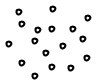
\includegraphics[width=0.2\textwidth]{seventeen.png}
\end{center}
It's just an \textit{amount}. There are more circles in that picture than
in some pictures, and less than in others. But in no way is it ``two
digits," nor do the particular digits ``1" and ``7" come into play any more
or less than any other digits. 

Let's keep thinking about this. Consider this number, which I'll label
``A":
\begin{center}
{\large (A)} \quad\quad \raisebox{-1cm}{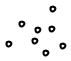
\includegraphics[width=0.15\textwidth]{eight.png}}
\end{center}
Now let's add another circle to it, creating a different number I'll call
``B":
\begin{center}
{\large (B)} \quad\quad
\raisebox{-1cm}{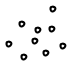
\includegraphics[width=0.15\textwidth]{nine.png}}
\end{center}
And finally, we'll do it one more time to get ``C":
\begin{center}
{\large (C)} \quad\quad
\raisebox{-1cm}{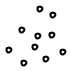
\includegraphics[width=0.15\textwidth]{ten.png}}
\end{center}
(Look carefully at those images and convince yourself that I added one
circle each time.)

When going from A to B, I added one circle. When going from B to C, I also
added one circle. Now I ask you: was going from B to C any more
``significant" than going from A to B? Did anything qualitatively different
happen? 

The answer is obviously no. Adding a circle is adding a circle; there's
nothing more to it than that. But if you had been writing these numbers out
as base-10 representations, like you're used to doing, you might have
thought differently. You'd have gone from:
\begin{center}
{\large (A)} \quad\quad \raisebox{-.6mm}{\LARGE 8}
\end{center}
to
\begin{center}
{\large (B)} \quad\quad \raisebox{-.6mm}{\LARGE 9}
\end{center}
to
\begin{center}
{\large (C)} \quad\quad \raisebox{-.6mm}{\LARGE 10}
\end{center}
When going from B to C, your ``odometer" wrapped around. You had to go from
a one-digit number to a two-digit number, simply because you ran out of
room in one digit. This can lead to the \textit{illusion} that something
fundamentally different happens when you go from B to C. \textit{This is
completely an illusion.} Nothing different happens to the \textit{number}
just because the way we write it down changes.

\index{odometer rollovers}
Human beings have a curious habit of thinking that odometer changes are
significant. When the temperature breaks 100, it suddenly feels ``more
hotter" than it did when it merely rose from 98 to 99. When the Dow Jones
Industrial Average first reached 10,000, and when Pete Rose eclipsed 4,000
career hits, and when the year 2000 dawned, we tended to think that
something truly important had taken place. But as we'll see, the point at
which these milestones occur is utterly and even laughably aribitrary: it
simply has to do with what number we've chosen as our \textit{base}. And we
quite honestly could have chosen any number at all.

\section{Bases}

\index{bases (of number systems)}
As I mentioned, a \textbf{base} is simply a number that's an anchor for our
place value system. It represents \textit{how many distinct symbols we
will use to represent numbers.} This implicitly sets the value of the
largest quantity we can hold in one digit, before we'd need to ``roll over"
to two digits.

\index{decimal numbers}
In base 10 (decimal), we use ten symbols: 0, 1, 2, 3, 4, 5, 6, 7, 8, and 9.
Consequently, the number nine is the highest value we can hold in a single
digit. Once we add another element to a set of nine, we have no choice but
to add another digit to express it. This makes a ``ten's place" because it
will represent the number of sets-of-10 (which we couldn't hold in the 1's
place) that the value contains.

Now why is the next place over called the ``hundred's place" instead of,
say, the ``twenty's place"? Simply because twenty --- as well as every
other number less than a hundred --- comfortably fits in two digits. We can
have up to 9 in the one's place, and also \textit{up to 9 in the ten's
place}, giving us a total of ninety-nine before we ever have to cave in to
using three digits. The number one hundred is exactly the point at which we
\textit{must} roll over to three digits; therefore, the sequence of digits
1-0-0 represents one hundred.

If the chosen base isn't obvious from context (as it often won't be in this
chapter) then when we write out a sequence of digits we'll append the base
as a subscript to the end of the number. So the number ``four hundred and
thirty-seven" will be written as $437_{10}$.

The way we interpret a decimal number, then, is by counting the right-most
digits as a number of \textit{individuals}, the digit to its left as the
number of \textit{groups of ten} individuals, the digit to \textit{its}
left as the number of groups of hundred individuals, and so on. $5472_{10}$
is just a way of writing $5 \times 1000 + 4 \times 100 + 7 \times 10 + 2
\times 1$.

\index{exponential notation}
If we use exponential notation (remember that anything to the
$0^{\text{th}}$ power is 1), this is equivalent to:
\[
5472_{10} = 5 \times 10^3 + 4 \times 10^2 + 7 \times 10^1 + 2 \times 10^0.
\]

\index{least significant digit}
\index{most significant digit}
By the way, we will often use the term \textbf{least significant digit} to
refer to the right-most digit (2, in the above example), and \textbf{most
significant digit} to refer to the left-most (5). ``Significant" simply
refers to how much that digit is ``worth" in the overall magnitude of the
number. Obviously 239 is less than 932, so we say that the hundreds place
is more significant than the other digits.

\index{bases (of number systems)}
All of this probably seems pretty obvious to you. All right then. Let's
use a base other than ten and see how you do. Let's write out a number
\textit{in base 7}. We have seven symbols at our disposal: 0, 1, 2, 3, 4,
5, and 6. Wait, you ask --- why not 7? Because there is no digit for seven
in a base 7 system, just like there is no digit for ten in a base 10
system. Ten is the point where we need \textit{two} digits in a decimal
system, and analogously, seven is the point where we'll need two digits in
our base 7 system. How will we write the value seven? Just like this:
\textbf{10}. Now stare at those two digits and practice saying ``seven" as
you look at them.  All your life you've been trained to say the number
``ten" when you see the digits 1 and 0 printed like that. But those two
digits only represent the number ten \textit{if you're using a base 10
system.} If you're using a base 34 system, ``10" is how you write
``thirty-four."

Very well, we have our seven symbols. Now how do we interpret a number like
$6153_7$? It's this:
\[
6153_{7} = 6 \times 7^3 + 1 \times 7^2 + 5 \times 7^1 + 3 \times 7^0.
\]
That doesn't look so strange: it's very parallel to the decimal string we
expanded, above. It looks weirder when we actually multiply out the place
values:
\[
6153_{7} = 6 \times 343 + 1 \times 49 + 5 \times 7 + 3 \times 1.
\]
So in base 7, we have a ``one's place," a ``seven's place," a
``forty-nine's place," and a ``three hundred forty-three's place." This
seems unbelievably bizarre --- how could a number system possibly hold
together with such place values? --- but I'll bet it wouldn't look funny at
all if we had been born with 7 fingers. Keep in mind that in the equation
above, we wrote out the place values as decimal numbers! Had we written
them as base-7 numbers (as we certainly would have if base 7 was our
natural numbering system), we would have written:
\[
6153_{7} = 6 \times 1000_7 + 1 \times 100_7 + 5 \times 10_7 + 3 \times 1_7.
\]
This is exactly equivalent numerically. Because after all, $1000_7$
\textit{is} $343_{10}$. A quantity that looks like an oddball in one base
system looks like the roundest possible number in another.


\section{Hexadecimal (base 16)}
\index{hexadecimal numbers}

Now objectively speaking, it turns out that ten is a pretty weird base too.
I know it doesn't seem like it, but that's only because we're so used to
it. Really, if you're repeatedly adding little circles to a drawing, ten is
a funny place to decide to draw the line and go to more digits. It's only
divisible by 2 and 5 (of all things), it's not a perfect square, and all
this makes it kind of an awkward choice.

\index{octal numbers}
In computer science, it turns out to be very (very) convenient to use a
base that is \textit{a power of two}. This means a base that is
``two-to-the-something." In earlier computing days, octal (base 8) was a
common choice. But for various reasons, that turns out to be less
convenient than using base 16, or \textbf{hexadecimal}.\footnote{Sometimes
numbers written in base 16 are called ``\textbf{hex numbers}."} Any time
you're working with hardware, operating systems, device drivers, bit masks,
or anything else low level, you'll encounter numbers written in base 16 a
heck of a lot. So let's study this particular base in some detail.

Base 16 will need sixteen digits, of course. Unfortunately, we
ten-fingered people have only invented ten symbols that are obviously
numerical: the digits 0 through 9. So what do we do for the other six?
It turns out that the originators of this system took perhaps the most
obvious approach: repurposing the letters of the alphabet. So we add the
``digits" A through F (sometimes written as capitals, sometimes in
lower-case) to our set of symbols. These, then, are the quantities that
each individual digit represents:
\begin{center}
\begin{tabular}{c l}
\texttt{0} & zero \\
\texttt{1} & one \\
\texttt{2} & two \\
\texttt{3} & three \\
\texttt{4} & four \\
\texttt{5} & five \\
\texttt{6} & six \\
\texttt{7} & seven \\
\texttt{8} & eight \\
\texttt{9} & nine \\
\texttt{A} & ten \\
\texttt{B} & eleven \\
\texttt{C} & twelve \\
\texttt{D} & thirteen \\
\texttt{E} & fourteen \\
\texttt{F} & fifteen \\
\end{tabular}
\end{center}
The inventors of hexadecimal notation didn't have to use the alphabet, of
course; they could have chosen a star for ten, a square for eleven, a happy
face for twelve, \textit{etc.}, but that wouldn't have been very easy to
type. So we're stuck with the letters, for better or for worse. Practice
staring at that letter \texttt{A} and saying the word ``ten." Because
that's what it means. In hexadecimal, the sequence of digits \texttt{10}
does \textit{not} mean ``ten." It means ``sixteen."

Those are the symbols. What are the place values? Well, they are (from the
right) the $16^0$'s place, the $16^1$'s place, the $16^2$'s place, and so
on. Written decimally, those work out to be the 1's place, the 16's place,
the 256's place, the 4096's place, and so on. Again, those numbers seem
strange only because when they are \textit{written decimally} they don't
come out very ``round."

The value of a number like 72E3 is computed as:
\[
\text{72E3}_{16} = 7 \times \text{4096}_{10} + 2 \times 256_{10} + 14 \times 16_{10} + 3
\times 1_{10} = \text{29,411}_{10}.
\]
Notice we treated the ``E" just like another digit, which it is. We also
called 72E3 ``a number," which it is. Get used to the idea that numbers ---
totally legitimate numbers --- can have letters for some of their digits.

In hexadecimal, what's the highest value that can fit in one digit?
Answer: \texttt{F} (which is fifteen.) What's the highest that can fit in
two digits? \texttt{FF} (which is two hundred fifty-five.) What about three
digits? \texttt{FFF} (which is sixty-five thousand five hundred
thirty-five.) And so on. If you count in hexadecimal, you do the same thing
as in decimal, only you ``roll over the odometer" when you get to F, not
when you get to 9.

\subsection{Converting to and from decimal}
\index{hexadecimal numbers}
\index{decimal numbers}

So we know how to take a hexadecimal number (like $\text{72E3}_{16}$) and
find its decimal equivalent: we just interpret each place's value as 1, 16,
256, 4096, and so on. What about going the other way? If we had a decimal
number, how would we write its value hexadecimally?

\index{modulo operator (mod)}
\index{remainder}
\index{quotient}
First, let's learn two operations (if you don't already know them) that
come in handy when working with integers. The first is called the
\textbf{modulo operator} (written ``\textbf{mod}"), and simply gives the
\textit{remainder} when dividing two numbers. This is a concept you
probably learned in elementary school but might not have used since then.
As we get older (and use calculators), we tend to think of a division
operation like $13 \div 3$ as being $4.333\dots$. But that's when we want a
real-valued (instead of integer-valued) answer. If we only want integers,
then we say that $13 \div 3$ is ``4 with a remainder of 1." (The ``4" is
called the \textbf{quotient}.) This means that if you have 13 objects, you
can take four groups of 3's out of them, and then have 1 object left over.
The way we write this operation mathematically is ``13 mod 3." In this
case, it turns out that 13 mod 3 = 1.

\index{congruent}
Let's think through what the mod operator yields for different values. We
know that 13 mod 3 = 1. What about 14 mod 3? That is equal to 2, since we
can (again) take out four groups of 3's, but then we'd have \textit{two}
left over. What about 15 mod 3? That yields 0, since 3 goes in to 15
evenly, leaving no remainder at all. 16 mod 3 again gives us 1, just like
13 did.  If you think it through, you'll realize that 19 mod 3 will also be
1, as will 22 mod 3 and 25 mod 3. These numbers that give the same
remainder are said to be ``\textbf{congruent} mod 3." The numbers 2, 5, 8,
11, 14, \textit{etc.} are also all congruent (to each other) mod 3, since
they all give a remainder of 2.

Another observation is that the value of $n$ mod $k$ always gives a value
between 0 and $k-1$. We may not know at a glance what 407,332,117 mod 3 is,
but we know it can't be 12, or 4, or even 3, because if we had that many
elements left after taking out groups of 3's, we could still take out
\textit{another} group of 3. The remainder only gives us what's left after
taking out groups, so by definition there cannot be an entire group (or
more) left in the remainder.

\index{floor operator ($\lfloor \ \rfloor$)}
The other operation we need is simply a ``round down" operation,
traditionally called ``\textbf{floor}" and written with brackets:
``$\lfloor \ \rfloor$". The floor of an integer is itself. The floor of a
non-integer is the integer just below it. So $\lfloor 7 \rfloor = 7$ and
$\lfloor 4.81 \rfloor = 4$. It's that simple.

\index{quotient}
\index{remainder}
The reason we use the floor operator is just to get the whole number of
times one number goes into another. $\lfloor 13 \div 3 \rfloor = 4$, for
example. By using mod and floor, we get the quotient and remainder of a
division, both integers. If our numbers are 25 and 7, we have $\lfloor 25
\div 7 \rfloor = 3$ and 25 mod 7 = 4. Notice that this is equivalent to
saying that $25 = 3 \times 7 + 4$. We're asking ``how many groups of 7 are
in 25?" and the answer is that 25 is equal to \textit{3} groups of 7, plus
4 extra.

The general procedure for converting from one base to another is to
repeatedly use mod and floor to strip out the digits from right to left. 
Here's how you do it:

\index{floor operator ($\lfloor \ \rfloor$)}
\index{modulo operator (mod)}
\vspace{.1in}
\begin{samepage}
\textbf{Express a numeric value in a base}
\label{convertalgorithm}
\begin{enumerate}
\item \label{modstep} Take the number mod the base. Write that digit down.
\item \label{divstep} Divide the number by the base and take the floor:
    \begin{enumerate}
    \item \label{zerostep} If you get zero, you're done.
    \item \label{notzerostep} If you get non-zero, then make this non-zero
number your new value, move your pencil to the left of the digit(s) you've
already written down, and return to step~\ref{modstep}.
    \end{enumerate}
\end{enumerate}
\end{samepage}
\vspace{.2in}

As an example, let's go backwards to the hex number 72E3 as in our example
above, which we already computed was equal to 29,411 in decimal. Starting
with 29,411, then, we follow our algorithm:

\begin{enumerate}

\item (Step~\ref{modstep}) We first compute 29,411 mod 16. This turns out
to be 3. Many scientific calculators can perform this operation, as can
programming languages like Java and data analysis languages like R. Or, you
could do long division (459,494 $\div$ 16) by hand and see what the
remainder is. Or, you could divide on an ordinary calculator and see
whether the part after the decimal point is 0, or $\frac{1}{16}^\text{th}$,
or $\frac{2}{16}^\text{ths}$, \textit{etc.} Or, you could sit there and
subtract 16 after 16 after 16 from 29,411 until there are no more 16's to
take out, and see what the answer is. At any rate, the answer is 3. So we
write down 3:

{\Large
\begin{center}
3
\end{center}
}

\item (Step~\ref{divstep}) We now divide 29,411 by 16 and take the floor.
This produces $\lfloor \text{29,411} \div 16 \rfloor = 1838$. Since this is
not zero, we perform step~\ref{notzerostep}: make 1838 our new value, move
our pencil to the left of the 3, and go back to step~\ref{modstep}.

\item (Step~\ref{modstep}) Now compute 1838 mod 16. This gives us the value
14, which is of course a base 10 number. The equivalent hex digit is E. So
we now write down E to the left of the 3:

{\Large
\begin{center}
E3
\end{center}
}

\item (Step~\ref{divstep}) Dividing 1838 by 16 and taking the floor gives
us 114. Since this is again not zero, we perform step~\ref{notzerostep}:
make 114 our new value, move our pencil to the left of the E, and go back
to step~\ref{modstep}.

\item (Step~\ref{modstep}) Next we compute 114 mod 16. This turns out to be
2, so we write down a 2:

{\Large
\begin{center}
2E3
\end{center}
}

\item (Step~\ref{divstep}) Computing $\lfloor 114 \div 16 \rfloor$ produces
7, which is again not zero, so 7 becomes our new value and we go back once
again to step~\ref{notzerostep}.

\item (Step~\ref{modstep}) 7 mod 16 is simply 7, so we write it down:

{\Large
\begin{center}
72E3
\end{center}
}

\item (Step~\ref{divstep}) Finally, $\lfloor 7 \div 16 \rfloor$ is zero, so
we go to step~\ref{zerostep} and we're done. The page has 72E3 written on
it in big bold letters, which is the correct answer.
\end{enumerate}

\subsection{Adding hex numbers}
\index{hexadecimal numbers}

Suppose we have two hexadecimal numbers, and we want to add them together
to get a hexadecimal result. How do we do it? One way is to first convert
them both to decimal, then add them like you learned in first grade, then
convert the answer back to hex. But we can stay ``natively hex" as long as
we add each pair of digits correctly.

Let's try it. Suppose we want to compute this sum:
\[
\begin{array}{*{5}{c@{\hspace{0pt}}}}
   &        4 &        8 & \text{D} & 4_{16} \\
 + &        5 &        9 &        2 & 5_{16} \\
\hline
   &          &          &          & ?_{16} \\
\end{array}
\]
We proceed in the first-grade way from right to left. Adding the
one's-place values, we get 4 + 5 = 9:
\[
\begin{array}{*{5}{c@{\hspace{0pt}}}}
   &        4 &        8 & \text{D} & 4_{16} \\
 + &        5 &        9 &        2 & 5_{16} \\
\hline
   &          &          &          & 9_{16} \\
\end{array}
\]
Easy enough. Now we add the next digit to the left (the sixteen's-place,
mind you, not the ten's place) and we find D + 2. Now what in the world is
``D+2"? It's actually easy: all you have to do is the same thing you did
when you were a child and you had to add something like 4 + 5. You hadn't
memorized the answer yet, and so you started with four fingers held up, and
counted off ``1\dots 2\dots 3\dots 4\dots 5," sticking up another finger
each time. Then, you looked at your hands, and behold! nine fingers.

We'll do the same thing here: start with the number ``D," and count two
additional places: ``E\dots F." The answer is F. That is the number that's
two greater than D. Lucky for us, it still fits in one digit. So now we
have:
\[
\begin{array}{*{5}{c@{\hspace{0pt}}}}
   &        4 &        8 & \text{D} & 4_{16} \\
 + &        5 &        9 &        2 & 5_{16} \\
\hline
   &          &          &        F & 9_{16} \\
\end{array}
\]
So far so good. The next pair of digits is 8 + 9. Here's where you want to
be careful. You're liable to look at ``8+9" and immediately say ``17!" But
8 + 9 is \textit{not} 17 in hexadecimal. To figure out
what it is, we start with the number 8, and count: ``9\dots A\dots B\dots
C\dots D\dots E\dots F\dots 10\dots 11\dots". The answer is ``11," which of
course is how you write ``seventeen" in hex. So just like in grade school,
we write down 1 and carry the 1:
\[
\begin{array}{*{5}{c@{\hspace{0pt}}}}
   &        \text{{\footnotesize 1}}  &          & & \\
   &        4 &        8 & \text{D} & 4_{16} \\
 + &        5 &        9 &        2 & 5_{16} \\
\hline
   &          &        1 &        F & 9_{16} \\
\end{array}
\]
Finally, our last digit is 4 + 5, plus the carried 1. We start with four
and count off five: ``5\dots 6\dots 7\dots 8\dots 9." Then we add the
carry, and count ``\dots A." The answer is A, with no carry, and so we have
our final answer:
\[
\begin{array}{*{5}{c@{\hspace{0pt}}}}
   &        \text{{\footnotesize 1}}  &          & & \\
   &        4 &        8 & \text{D} & 4_{16} \\
 + &        5 &        9 &        2 & 5_{16} \\
\hline
   & \textbf{A} & \textbf{1} & \textbf{F} & \textbf{9}_{\textbf{16}} \\
\end{array}
\]


\section{Binary (base 2)}
\index{binary numbers}
\index{bit}

The other base we commonly use in computer science is base 2, or
\textbf{binary}. This is because the basic unit of information in a
computer is called a \textbf{bit}, which has only two values,
conventionally called either ``true" and ``false" or ``1" and ``0". Numbers
(as well as everything else) are ultimately represented as colossal
sequences of 1's and 0's, which are of course binary numbers.

The rules for interpreting place value are the same:
\begin{align*}
\text{110101}_{2} &= 
1 \times 2^5 + 
1 \times 2^4 + 
0 \times 2^3 + 
1 \times 2^2 + 
0 \times 2^1 + 
1 \times 2^0 \\
&= 1 \times 32 + 
1 \times 16 + 
0 \times 8 + 
1 \times 4 + 
0 \times 2 + 
1 \times 1 \\
&= \text{53}_{10}.
\end{align*}
\index{least significant bit (LSB)}
\index{most significant bit (MSB)}
So in binary we have a one's-place, a two's-place, a four's-place, an
eight's-place, and so on. We call the right-most place the \textbf{least
significant bit (LSB)} and the left-most the \textbf{most significant bit
(MSB)}.

Counting up from zero is really just the same as any other base, although
it feels a little strange in binary because you ``roll over" so often:
\begin{center}
\begin{tabular}{r l}
$\texttt{0}_2$ & zero \\
$\texttt{1}_2$ & one \\
$\texttt{10}_2$ & two \\
$\texttt{11}_2$ & three \\
$\texttt{100}_2$ & four \\
$\texttt{101}_2$ & five \\
$\texttt{110}_2$ & six \\
$\texttt{111}_2$ & seven \\
$\texttt{1000}_2$ & eight \\
$\texttt{1001}_2$ & nine \\
\vdots & \vdots
\end{tabular}
\end{center}


\subsection{Converting to and from decimal}
\index{decimal numbers}
\index{binary numbers}

Converting from binary to decimal was demonstrated above (with
$110101_2=53_{10}$.) To go the other way, we follow the algorithm from
page~\pageref{convertalgorithm}. Let's try it for the decimal number 49:

\begin{enumerate}
\item (Step~\ref{modstep}) We first compute 49 mod 2. Doing ``mod 2" is
easy: you just see whether the number is even or odd. In this case, it's
odd, so the remainder is a 1:

{\Large
\begin{center}
1
\end{center}
}

\item (Step~\ref{divstep}) Now divide 49 by 2 and take the floor, which
gives $\lfloor \text{49} \div 2 \rfloor = 24$. It's not zero, so
we perform step~\ref{notzerostep}: make 24 our new value, move
our pencil to the left of the 1, and go back to step~\ref{modstep}.

\item (Step~\ref{modstep}) Compute 24 mod 2. Since 24 is even, this is
zero, which we write down to the left of the 1:

{\Large
\begin{center}
01
\end{center}
}

\item (Step~\ref{divstep}) Divide 24 by 2 and take the floor, which gives
$\lfloor \text{24} \div 2 \rfloor = 12$.  Make 12 our new value, move our
pencil to the left of the 0, and go back to step~\ref{modstep}.

\item (Step~\ref{modstep}) Compute 12 mod 2. Since 12 is even, this is
zero, which we write down:

{\Large
\begin{center}
001
\end{center}
}

\item (Step~\ref{divstep}) Divide 12 by 2 and take the floor, which gives
$\lfloor \text{12} \div 2 \rfloor = 6$.  Make 6 our new value, move our
pencil to the left of the 0, and go back to step~\ref{modstep}.

\item (Step~\ref{modstep}) Compute 6 mod 2. Since 6 is even, this is
zero, which we write down:

{\Large
\begin{center}
0001
\end{center}
}

\item (Step~\ref{divstep}) Divide 6 by 2 and take the floor, which gives
$\lfloor \text{6} \div 2 \rfloor = 3$.  Make 3 our new value, move our
pencil to the left of the 0, and go back to step~\ref{modstep}.

\item (Step~\ref{modstep}) Compute 3 mod 2. Since 3 is odd, this is
one, which we write down:

{\Large
\begin{center}
10001
\end{center}
}

\item (Step~\ref{divstep}) Divide 3 by 2 and take the floor, which gives
$\lfloor \text{3} \div 2 \rfloor = 1$.  This still isn't zero, so make 1
our new value, move our pencil to the left of the 0, and go back to
step~\ref{modstep}.

\item (Step~\ref{modstep}) Compute 1 mod 2. Since 1 is odd, this is
one, which we write down:

{\Large
\begin{center}
110001
\end{center}
}

\item (Step~\ref{divstep}) Divide 1 by 2 and take the floor, which gives
$\lfloor \text{1} \div 2 \rfloor = 0$.  We're done. The final answer is
$110001_2$. Double-checking our work, we verify that indeed one 32 plus one
16 plus one 1 gives 49, which is what we started with.
\end{enumerate}


\subsection{Converting to and from hex}
\index{hexadecimal numbers}
\index{binary numbers}

That was pretty tedious. But converting back and forth from binary to
\textit{hex} is a snap. That's because 16 is exactly $2^4$, and so one hex
digit is exactly equal to four binary digits. This isn't the case with base
10, where one decimal digit is equal to three binary digits\dots
\textit{plus} a little extra. This ``not quite a whole number of digits"
thing is what makes converting from decimal to binary (or decimal to hex,
for that matter) so awkward.

\index{byte}
We most commonly deal with sets of eight bits at a time, which is called a
\textbf{byte}. (This is the fundamental unit of storage on pretty much
every computer on earth.) Suppose I had the following byte:
\begin{center}
{\large
$\texttt{10000110}_2$
}
\end{center}
Because one hex digit is exactly equal to four bits, this byte is exactly
equal to:
\begin{center}
{\large
$\texttt{86}_{16}$
}
\end{center}
\index{nibble}
This is because the byte can be neatly split into two parts: \texttt{1000},
which corresponds to the hex digit 8, and 0110, which corresponds to the
hex digit 6. These two halves are called \textbf{nibbles} --- one byte has
two nibbles, and each nibble is one hex digit. At a glance, therefore, with
no multiplying or adding, we can convert from binary to hex.

Going the other direction is just as easy. If we have:
\begin{center}
{\large
$\texttt{3E}_{16}$
}
\end{center}
we just convert each hex digit into the corresponding nibble:
\begin{center}
{\large
$\texttt{00111110}_2$
}
\end{center}
After you do this a while, you get to the point where you can instantly
recognize which hex digit goes with which nibble value. Until then, though,
here's a handy table:
\begin{center}
\begin{tabular}{|c|c|}
\hline
nibble & hex digit \\
\hline
\texttt{0000} & \texttt{0} \\
\texttt{0001} & \texttt{1} \\
\texttt{0010} & \texttt{2} \\
\texttt{0011} & \texttt{3} \\
\texttt{0100} & \texttt{4} \\
\texttt{0101} & \texttt{5} \\
\texttt{0110} & \texttt{6} \\
\texttt{0111} & \texttt{7} \\
\texttt{1000} & \texttt{8} \\
\texttt{1001} & \texttt{9} \\
\texttt{1010} & \texttt{A} \\
\texttt{1011} & \texttt{B} \\
\texttt{1100} & \texttt{C} \\
\texttt{1101} & \texttt{D} \\
\texttt{1110} & \texttt{E} \\
\texttt{1111} & \texttt{F} \\
\hline
\end{tabular}
\end{center}
In case you're wondering, yes this is worth memorizing.


\subsection{Adding binary numbers}
\index{binary numbers}

Adding two binary numbers is the same as adding in decimal, hexadecimal, or
any other base: you just have to know when to ``roll over the odometer,"
which in this case is almost instantly, since the highest value a bit can
hold is 1! Let's give it a shot:
\[
\begin{array}{*{7}{c@{\hspace{0pt}}}}
%   & \text{{\footnotesize 1}}  &          & & \\
   & \texttt{1} & \texttt{1} & \texttt{1} & \texttt{0} & \texttt{0} & \texttt{1}_2 \\
 + & \texttt{0} & \texttt{1} & \texttt{1} & \texttt{0} & \texttt{1} & \texttt{0}_2 \\
\hline
   & \texttt{ } & \texttt{ } & \texttt{ } & \texttt{ } & \texttt{ } & \texttt{?}_2 \\
\end{array}
\]
A child could follow the rules: when we add two zeroes, we get zero. Adding
a one to a zero gives one. Adding two ones gives zero, and a carry to the
next significant digit. And adding two ones plus a carry gives a one and a
carry. See if you can follow the flow:
\[
\begin{array}{*{7}{c@{\hspace{0pt}}}}
   & \texttt{{\footnotesize 1}}  & \texttt{{\footnotesize 1}}         & & \\
   & \texttt{1} & \texttt{1} & \texttt{1} & \texttt{0} & \texttt{0} & \texttt{1}_2 \\
 + & \texttt{0} & \texttt{1} & \texttt{1} & \texttt{0} & \texttt{1} & \texttt{0}_2 \\
\hline
 \texttt{1} & \texttt{0} & \texttt{1} & \texttt{0} & \texttt{0} & \texttt{1} & \texttt{1}_2 \\
\end{array}
\]

\subsection{Capacity}
\index{capacity (of a byte)}

How large a value can a byte store? There are 8 bits, and each one can
independently have either of two values (0 or 1), so by the Fundamental
Theorem of Counting, there are $2^8$ different combinations. This works out
to 256, but we can't actually store the number 256 in a byte if we're using
the bit pattern $\texttt{00000000}_2$ (or $\texttt{00}_{16}$) to represent
zero. The highest value would be$\texttt{11111111}_2$ (or
$\texttt{FF}_{16}$), which is $256_{10}$.

How do we store a number larger than that? Simply use more than one byte,
of course. If we used two bytes of memory, and treated them as concatenated
one after the other, that would give us 16 bits, allowing us to store up to
the number $\texttt{0000000000000000}_2$ = $\texttt{FFFF}_{16}$ =
$\text{65,535}_{10}$. We'd call one of these bytes --- the one representing
the $2^0$'s place up to the $2^7$'s place --- the least significant
\textit{byte}, and the other one --- containing places $2^8$ through
$2^{15}$ --- the most significant byte. Extending to more than two bytes to
accommodate even larger numbers is done in the obvious way.


\subsection{Binary representation schemes}
\index{negative numbers (in binary)}

That's mostly all there is to it. But there's one thing we haven't
discussed yet, and that's \textit{negative} numbers. We know how to
represent any positive number (or zero) with an ordinary place value
scheme. But how do we store a number like $-5$?

There are three different schemes for treating negative numbers, each with
its strengths and weaknesses.

\subsubsection{Unsigned}
\index{unsigned binary numbers}

The simplest scheme is called \textbf{unsigned}, and it simply means that
we don't \textit{allow} negative numbers. For one byte, we have 256
different bit patterns at our disposal, and we might just choose to
allocate them all to represent positive numbers, so as to get the widest
range. This makes sense for, say, a C++ program variable called
\texttt{heightInInches} which we know can never meaningfully be negative
(no one has a negative height).

The advantage of this scheme is simply that we can represent the greatest
possible range of positive numbers, which is sometimes the goal. Each of
the alternative schemes carves off a chunk of these available bit patterns
and devotes them to representing negative numbers, leaving fewer left over
for positive numbers. There's no free lunch: you have to decide how you
want to ``spend" your available bit patterns depending on what values you
need to represent.

\subsubsection{Sign-magnitude}
\index{sign-magnitude binary numbers}

The \textbf{sign-magnitude} scheme is probably the first thing you'd think
of to solve the negative number representation problem. We need to store
the sign of the number somehow, and a sign is inherently a two-valued thing
(either positive or negative), so why not peel off one of the bits and use
it to represent the sign? The remaining bits can then be used in the
ordinary way to represent the magnitude of the number.

The way this is most often done is to take the left-most bit and use it as
the \textbf{sign bit}. This bit now has \textit{no other meaning}. It can't
``double" as the 128's place, because then there'd be no way to distinguish
between, say, 129 and $-129$ (each would be represented with
\texttt{10000001}.) No, the sign bit must be considered ``spent money," and
its expressive power cannot be reclaimed to also represent part of the
magnitude. By convention, if the sign bit is 0 this represents a
\textit{positive} number, and a sign bit of 1 represents a
\textit{negative} number. (That might seem counterintuitive, but hey,
that's the way it is.)

So this number in sign-magnitude:
\begin{center}
{\large
\textbf{0}0100110
}
\end{center}
represents the decimal number 38. That's because the sign bit (bolded, on
the far left) is 0, which means the number is positive. The magnitude of
the number is contained in the other 7 bits, which gives 32 + 4 + 2 = 38.
This number, on the other hand:
\begin{center}
{\large
\textbf{1}0100110
}
\end{center}
represents $-38$. The magnitude is the same, but the sign bit is 1 so this
pattern now ``means" a negative number.

Clearly we have reduced our range of positive numbers in exchange for the
ability to also store negatives. We have 7 bits of range instead of 8, so
instead of 255, our highest possible value is merely 127. On the other end,
the lowest possible value is $-127$. 

If you have sharp eyes, you may have noticed a discrepancy in the counting.
With the sign-magnitude approach, we can hold numbers in the range $-127$
to 127. But wait: that's only 255 different values, not 256! Why did we
lose one value of expressive power? The answer is that the sign-magnitude
scheme has \textit{two ways} of representing \textit{zero}. The bit
pattern \texttt{00000000} is obviously zero, but so is \texttt{10000000}
(which you might call ``negative zero.") Using two different patterns to
represent the same value is a little wasteful, but the situation is
actually worse than that. Having to account for both patterns means that
computer hardware using the sign-magnitude scheme is inevitably more
complicated. To compare two bytes to see if they're equal, you'd think we'd
just compare each bit position, and if they were all the same, the bytes
would be declared equal, otherwise no. Alas, this is no longer quite that
simple. The two zero patterns must be considered numerically equal, so our
digital logic now has to contain a special case. ``To be equal, all the
bits have to be the same\dots oh, but actually not if the right-most seven
are all zeroes in both bytes. In that case, it doesn't matter what the
left-most bit contains." Maddening.

\subsubsection{Two's-complement}
\index{two's-complement binary numbers}

This shortcoming in the sign-magnitude scheme is remedied with the
\textbf{two's-complement} scheme, which is the one actually used most often
in practice. It'll seem weird at first --- certainly not as intuitive as
the first two --- but it leads to a critically important feature that we'll
look at shortly.

First, the rules. To interpret a two's-complement number, you:
\begin{enumerate}
\item Look at the left-most bit (just like in sign-magnitude). If it's a 0,
you have a positive number. If it's a 1, you have a negative number.
\item If it's a positive number, the other 7 bits give you the magnitude
(just like in sign-magnitude).
\item If, however, it's a negative number, then to discover the magnitude
of that negative number you must \textit{flip all the bits and add one}.
This will give you a positive number which is the absolute value of your
negative number.
\end{enumerate}
Easy example: take the byte \texttt{00100110}. The left-most bit is a 0,
which means it's a positive number, and as we discovered above, the
remaining 7 bits give a magnitude of 38. So this is the number 38.

Harder example: take the byte \texttt{10100110}. The left-most bit is a 1,
which means it's negative. Okay: negative \textit{what}? How do we find the
magnitude? Well, we ``flip" all the bits (\textit{i.e.}, invert each one
from 0 to 1 or vice versa) to get:
\[
\begin{array}{*{8}{c@{\hspace{0pt}}}}
 \texttt{0} & \texttt{1} & \texttt{0} & \texttt{1} & \texttt{1} & \texttt{0} & \texttt{0} & \texttt{1} \\
\end{array}
\]
and then add one to the result:
\[
\begin{array}{*{9}{c@{\hspace{0pt}}}}
&  & & & & & & \texttt{{\footnotesize 1}} & \\
 & \texttt{0}  & \texttt{1} & \texttt{0} & \texttt{1} & \texttt{1} & \texttt{0} & \texttt{0} & \texttt{1} \\
 + & & \texttt{ } & \texttt{ } & \texttt{ } & \texttt{ } & \texttt{ } & \texttt{ } & \texttt{1} \\
\hline
 & \texttt{0} &  \texttt{1} & \texttt{0} & \texttt{1} & \texttt{1} & \texttt{0} & \texttt{1} & \texttt{0} \\
\end{array}
\]
This black magic produces the value $\texttt{01011010}_2$, which converts to
$90_{10}$. \textbf{This means that the original number, \texttt{10100110}, corresponds to the
value --90.}

``Flipping all the bits and adding one" is the cookbook procedure for
taking the complement (negative) of a number in the two's-complement
scheme. It works in reverse, too. Let's start with 90 this time and crank through
the process again, making sure we get --90.

Start with the binary representation of $90_{10}$:
\[
\begin{array}{*{8}{c@{\hspace{0pt}}}}
 \texttt{0} & \texttt{1} & \texttt{0} & \texttt{1} & \texttt{1} & \texttt{0} & \texttt{1} & \texttt{0} \\
\end{array}
\]
Flip all the bits to get:
\[
\begin{array}{*{8}{c@{\hspace{0pt}}}}
 \texttt{1} & \texttt{0} & \texttt{1} & \texttt{0} & \texttt{0} & \texttt{1} & \texttt{0} & \texttt{1} \\
\end{array}
\]
and finally add one to the result:
\[
\begin{array}{*{9}{c@{\hspace{0pt}}}}
&  & & & & & & \texttt{{\footnotesize 1}} & \\
 & \texttt{1}  & \texttt{0} & \texttt{1} & \texttt{0} & \texttt{0} & \texttt{1} & \texttt{0} & \texttt{1} \\
 + & & \texttt{ } & \texttt{ } & \texttt{ } & \texttt{ } & \texttt{ } & \texttt{ } & \texttt{1} \\
\hline
 & \texttt{1} &  \texttt{0} & \texttt{1} & \texttt{0} & \texttt{0} & \texttt{1} & \texttt{1} & \texttt{0} \\
\end{array}
\]
We get \texttt{10100110}, which was precisely the number we originally
began with, and which we have already determined represents --90.

Now you may ask what we gain from all this. Surely this scheme is
considerably more convoluted than the simple idea of reserving one bit as a
sign bit, and treating the rest as a magnitude. But it turns out there is
indeed a method to the madness. Strange as it sounds, a two's-complement
representation scheme allows us to \textit{perform addition and subtraction
with a single operation.}

In first grade (or so), you learned the procedure for adding multi-digit
numbers, which we've followed several times in this chapter. It involves
adding the digits right-to-left and possibly ``carrying." Then in second
grade (or so), you learned the procedure for \textit{subtracting}
multi-digit numbers. It involves subtracting the digits right-to-left and
possibly ``borrowing." If you're like me, you found adding easier than
subtracting. It's easy to just carry the one, but to borrow requires
looking at the digit to the left, making sure that you \textit{can} borrow
from it (\textit{i.e.}, that it's not already 0), borrowing from further
left until you actually find an available non-zero value, hoping the number
on the bottom is actually less than the one on the top (because otherwise
you have to switch the order and then add a negative sign to the result),
and keeping all of that straight as you march down the line. 

Even if you didn't find subtracting more difficult than adding, though, you
can't argue that it's still a completely \textit{different} algorithm, with
different rules to follow. In computer hardware, we have to implement
different circuitry to perform each operation, which is more difficult,
costly, error-prone, and power-draining.

The wonderful thing about two's-complement, however, is that with this
scheme we actually \textit{never need to use the subtraction algorithm.} If
we want to subtract two numbers --- say, $24 - 37$ --- we can instead take
the complement of the second number and then add them. Instead of $24-37$
we compute $24 + (-37)$. 

Let's see it in action. Using conversion procedures, we can figure out that
$24_{10}$ is:
\[
\begin{array}{*{8}{c@{\hspace{0pt}}}}
 \texttt{0} & \texttt{0} & \texttt{0} & \texttt{1} & \texttt{1} & \texttt{0} & \texttt{0} & \texttt{0} \\
\end{array}
\]
and that \textit{positive} $37_{10}$ is:
\[
\begin{array}{*{8}{c@{\hspace{0pt}}}}
 \texttt{0} & \texttt{0} & \texttt{1} & \texttt{0} & \texttt{0} & \texttt{1} & \texttt{0} & \texttt{1} \\
\end{array}
\]
If we wanted to compute $24+37$, we'd just add these. But instead
we're looking for $24-37$, so we'll take the complement of 37 to find
$-37$. Flip all the bits of 37:
\[
\begin{array}{*{8}{c@{\hspace{0pt}}}}
 \texttt{1} & \texttt{1} & \texttt{0} & \texttt{1} & \texttt{1} & \texttt{0} & \texttt{1} & \texttt{0} \\
\end{array}
\]
and add one:
\[
\begin{array}{*{9}{c@{\hspace{0pt}}}}
 \texttt{1} & \texttt{1} & \texttt{0} & \texttt{1} & \texttt{1} & \texttt{0} & \texttt{1} & \texttt{0} \\
 + & \texttt{ } & \texttt{ } & \texttt{ } & \texttt{ } & \texttt{ } & \texttt{ } & \texttt{1} \\
\hline
 \texttt{1} & \texttt{1} & \texttt{0} & \texttt{1} & \texttt{1} & \texttt{0} & \texttt{1} & \texttt{1} \\
\end{array}
\]
and so now we've determined that in the two's-complement scheme, $-37$ is
represented by $\texttt{11011011}_2$.

We're now ready to compute $24 + (-37)$:
\[
\begin{array}{*{9}{c@{\hspace{0pt}}}{l}}
& &   & \texttt{{\footnotesize 1}} & \texttt{{\footnotesize 1}} & & & & \\
   & \texttt{0} & \texttt{0} & \texttt{0} & \texttt{1} & \texttt{1} & \texttt{0} & \texttt{0} & \texttt{0} 
& \quad \textsl{$\leftarrow$ this is $24_{10}$}\\
 + & \texttt{1} & \texttt{1} & \texttt{0} & \texttt{1} & \texttt{1} & \texttt{0} & \texttt{1} & \texttt{1} 
& \quad \textsl{$\leftarrow$ this is $-37_{10}$}\\
\hline
   & \texttt{1} & \texttt{1} & \texttt{1} & \texttt{1} & \texttt{0} & \texttt{0} & \texttt{1} & \texttt{1} & \\
\end{array}
\]
%Notice that I put the left-most carried-over 1 of the answer in
%parentheses. More on that later. For now, the rule is ``we simply discard
%anything that carries over off the left end."

So we have our two's-complement answer, \texttt{11110011}. What value
does that correspond to? Well, the left-most bit is a 1, so it's a negative
number. To find out what it's the negative \textit{of}, flip all the bits
and add one:
\[
\begin{array}{*{8}{c@{\hspace{0pt}}}{l}}
 \texttt{0} & \texttt{0} & \texttt{0} & \texttt{0} & \texttt{1} & \texttt{1} & \texttt{0} & \texttt{0} 
& \quad \textsl{$\leftarrow$ flip the bits to get}\\
 + & \texttt{ } & \texttt{ } & \texttt{ } & \texttt{ } & \texttt{ } & \texttt{ } & \texttt{1} 
& \quad \textsl{$\leftarrow$ add one}\\
\hline
 \texttt{0} & \texttt{0} & \texttt{0} & \texttt{0} & \texttt{1} & \texttt{1} & \texttt{0} & \texttt{1} \\
\end{array}
\]
This is positive 13, which means the number we inverted to get it ---
\texttt{11110011} --- must represent $-13$. And that is indeed the
correct answer, for $24-37=-13$.

One last word on two's-complement: what is the \textit{range} of numbers we
can represent? It turns out to be -128 to 127. The highest value is
\texttt{01111111}, which is 127. You might think the lowest value would be
represented as \texttt{11111111}, but if you work it out, you'll find that
this is actually the number $-1$. The lowest number is actually the bit
pattern \texttt{10000000}, which is $-128$.

\subsection{Overflow}
\index{overflow}

One last sticky detail we need to cover has to do with \textbf{overflow}.
When we add two numbers, there is the possibility that the result will
contain one more digit than the original numbers did. You've probably seen
this on a hand calculator when you press ``=" and get an ``\texttt{E}" (for
``error") in the display. If there are only ten digits on your display,
adding two ten-digit numbers will (sometimes) result in an eleven-digit
number that your calculator can't display, and it's alerting you to that
fact so you don't misinterpret the result. Here, we might add two 8-bit
quantities and end up with a 9-bit quantity that can't fit in one byte.
This situation is called overflow, and we need to detect when it occurs.

\index{unsigned binary numbers}
The rules for detecting overflow are different depending on the scheme.
For \textit{unsigned} numbers, the rule is simple: if a 1 is carried out
from the MSB (far left-side), then we have overflow. So if I were to try to
add $155_{10}$ and $108_{10}$:
\[
\begin{array}{*{9}{c@{\hspace{0pt}}}{l}}
  & \texttt{{\footnotesize 1}} & \texttt{{\footnotesize 1}} & \texttt{{\footnotesize 1}} & \texttt{{\footnotesize 1}} & & & & \\
  & \texttt{1} & \texttt{0} & \texttt{0} & \texttt{1} & \texttt{1} & \texttt{0} & \texttt{1} & \texttt{1} 
& \quad \textsl{$\leftarrow$ $155_{10}$}\\
+ & \texttt{0} & \texttt{1} & \texttt{1} & \texttt{0} & \texttt{1} & \texttt{1} & \texttt{0} & \texttt{0} 
& \quad \textsl{$\leftarrow$ $108_{10}$}\\
\hline
\texttt{1} & \texttt{0} & \texttt{0} & \texttt{0} & \texttt{0} & \texttt{1} & \texttt{1} & \texttt{1} & \texttt{1} \\
\end{array}
\]
then I get a carry out left into the 9th digit. Since we can only hold eight
digits in our result, we would get a nonsensical answer ($15_{10}$), which
we can detect as bogus because the carry out indicated overflow.

\index{sign-magnitude binary numbers}
Sign-magnitude works the same way, except that I have one fewer bit when
I'm adding and storing results. (Instead of a byte's worth of bits
representing magnitude, the left-end bit has been reserved for a special
purpose: indicating the number's sign. Therefore, if I add the remaining
7-bit quantities and get a carry out left into the \textit{eighth} digit,
that would indicate overflow.)

\index{two's-complement binary numbers}
\index{carry-in}
\index{carry-out}
Now with two's-complement, things are (predictably) not that easy. But it
turns out they're \textit{almost} as easy. There's still a simple rule to
detect overflow, it's just a different rule. The rule is: if the carry
\textit{in to} the last (left-most) bit is \textit{different} than the
carry \textit{out from} the last bit, then we have overflow.

Let's try adding $103_{10}$ and $95_{10}$ in two's-complement, two numbers
which fit in our -128 to 127 range, but whose sum will not:
\[
\begin{array}{*{9}{c@{\hspace{0pt}}}{l}}
{\footnotesize \text{carry-in}} \rightarrow & \texttt{{\footnotesize 1}} & \texttt{{\footnotesize 1}} & \texttt{{\footnotesize 1}}  & \texttt{{\footnotesize 1}} & \texttt{{\footnotesize 1}} & \texttt{{\footnotesize 1}} & \texttt{{\footnotesize 1}} & \\
  & \texttt{0} & \texttt{1} & \texttt{1} & \texttt{0} & \texttt{0} & \texttt{1} & \texttt{1} & \texttt{1} 
& \quad \textsl{$\leftarrow$ $103_{10}$}\\
\quad + & \texttt{0} & \texttt{1} & \texttt{0} & \texttt{1} & \texttt{1} & \texttt{1} & \texttt{1} & \texttt{1} 
& \quad \textsl{$\leftarrow$ $95_{10}$}\\
\hline
{\footnotesize \text{carry-out}} \rightarrow \texttt{0} & \texttt{1} & \texttt{1} & \texttt{0} & \texttt{0} & \texttt{0} & \texttt{1} & \texttt{1} & \texttt{0} \\
\end{array}
\]
The carry-in to the last bit was 1, but the carry-out was 0, so for
two's-complement this means we detected overflow. It's a good thing, too,
since \texttt{11000110} in two's-complement represents $-57_{10}$, which is
certainly not 103 + 95.

Essentially, if the carry-in is not equal to the carry-out, that means we
added two positive numbers and came up with a negative number, or that we
added two negatives and got a positive. Clearly this is an erroneous
result, and the simple comparison tells us that. Just be careful to realize
that the rule for detecting overflow depends \textit{totally} on the
particular representation scheme we're using. A carry-out of 1 always means
overflow\dots \textit{in the unsigned scheme.} For two's-complement, we can
easily get a carry-out of 1 with no error at all, provided the carry-in is
\textit{also} 1.

\subsection{``It's all relative"}

Finally, if we come up for air out of all this mass of details, it's worth
emphasizing that there is no intrinsically ``right" way to interpret a
binary number. If I show you a bit pattern --- say, \texttt{11000100} ---
and ask you what value it represents, you can't tell me without knowing how
to interpret it.

If I say, ``oh, that's an unsigned number," then you'd treat each bit as a
digit in a simple base 2 numbering scheme. You'd add $2^7 + 2^6 + 2^2$ to
get 196, then respond, ``ah, then that's the number $196_{10}$." And you'd
be right.

But if I say, ``oh, that's a sign-magnitude number," you'd first look at
the leftmost bit, see that it's a 1, and realize you have a negative
number. Then you'd take the \textit{remaining} seven bits and treat them
as digits in a simple base 2 numbering scheme. You'd add $2^6 + 2^2$ to get
68, and then respond, ``ah, then that's the number $-68_{10}$." And you'd
be right.

But then again, if I say, ``oh, that's a two's-complement number," you'd
first look at the leftmost bit, see that it's a 1, and realize you're
dealing with a negative number. What is it the negative of? You'd flip all
the bits and add one to find out. This would give you $\texttt{00111100}$,
which you'd interpret as a base 2 number and get $60_{10}$. You'd then
respond, ``ah, then that's the number $-60_{10}$." And you'd be right.

So what does \texttt{11000100} represent then?? Is it 196, $-68$, or $-60$?
The answer is \textit{any of the three}, depending on what representation
scheme you're using. None of the data in computers or information systems
has intrinsic meaning: it all has to be interpreted according to the
syntactic and semantic rules that we invent. In math and computer science,
anything can be made to mean anything: after all, we invent the rules.
